\chapter{Validación en simulador}
\label{ch:simulation-implementation}

El entorno de simulación que nos ofrece \gls{sumo}\index{SUMO} nos permite recoger la práctica totalidad de información propuesta en la Tabla~\ref{tbl:main-variables} del capítulo \nameref{ch:methodology} con la excepción del entorno. El problema es que la representación que nos ofrece \gls{sumo}\index{SUMO} de éste es un conjunto posiciones y tipologías de elementos, de tal manera que podemos acceder a información rápidamente pero de forma muy limitada.

La solución por la que se ha optado es por la implementación de un \acrshort{lidar}\index{LiDAR} en el vehículo simulado de tal manera que ofrece una nube de puntos de las mismas características que las capturadas por el \acrshort{lidar}\index{LiDAR} físico y situado en la misma posición del vehículo. Este \acrshort{lidar}\index{LiDAR}, a una frecuencia de \SI{10}{\hertz}, realizará las siguientes operaciones:

\begin{enumerate}
	\item Captura de posición de todos los vehículos situados a un radio $r$ del centro del \acrshort{lidar}\index{LiDAR} y transformación de éstos a prismas con las dimensiones que especifiquen sus propiedades.
	\item Cálculo de la nube de puntos colisionando contra dichos prismas.
\end{enumerate}

\begin{marginfigure}
	\centering
	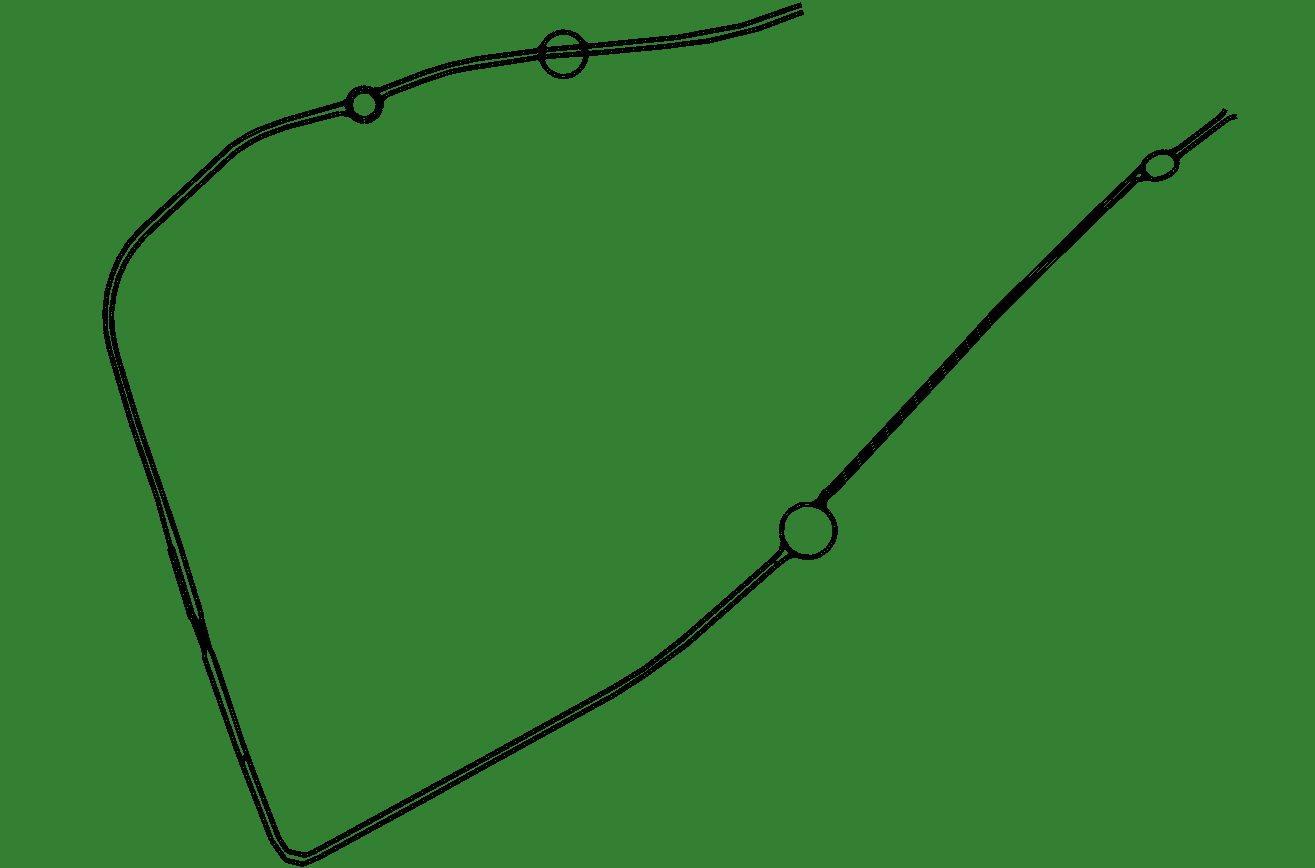
\includegraphics[width=\textwidth]{sumo-route}
	\caption[Circuito de prueba en el entorno virtual]{Circuito generado para recoger los datos de los vehículos circulando con los modelos longitudinal y de cambio de carril implantados.}
	\label{fig:sumo-route}
\end{marginfigure}

En el vehículo se han implantado los modelos longitudinales y de cambio de carril\index{lane-change} dentro de un conductor virtual, tanto para el sujeto global como para cada uno de los sujetos del experimento (identificados con la misma notación: $S_A$, $S_1$, $S_2$ y $S_3$). Posteriormente se ha realizado un recorrido de características similares al recorrido del que se obtuvieron los datos del conjunto de test (ver Figura~\ref{fig:sumo-route}).

Por último, se ha realizado el mismo recorrido en iguales condiciones con el modelo de conductor proporcionado por defecto por \gls{sumo}\index{SUMO}, al cual se le notará como $S_S$. Los valores para sus parámetros de configuración se describen en la Tabla~\ref{tbl:default-driver-config}).

\begin{table}
	\centering
	\caption[Indicadores reales frente a indicadores capturados en simulación]{Indicadores reales frente a indicadores capturados en simulación.}
	\label{tbl:default-driver-config}
	\begin{tabularx}{\linewidth}{cY}
		\toprule
		Parámetro & Valor \\
		\midrule
		\rowcolor{black!20} Aceleración (\SI{}{\meter\per\square\second}) & $0.2$ \\
		                    Deceleración (\SI{}{\meter\per\square\second}) & $-0.2$ \\
		\rowcolor{black!20} Velocidad máxima (\SI{}{\meter\per\second}) & $13$ \\
                            Imperfección ($\in [0, 1]$) & $0.5$ \\
		\rowcolor{black!20} Ancho (\SI{}{\meter}) & $1.475$ \\
                            Largo (\SI{}{\meter}) & $3.475$ \\
		\bottomrule
	\end{tabularx}
\end{table}

Estos valores se han elegido para asemejarse en la medida de lo posible a los valores obtenidos del conductor general. La aceleración y deceleración se han aproximado a aquellos valores obtenidos de las pruebas reales. La velocidad máxima de la máxima existente en el recorrido. El ancho y el alto de las especificaciones del vehículo real.

Por último, la imperfección del conductor se ha escogido a partir del valor recomendado en \cite{krauss1998microscopic}. De esta manera se comprobará si los datos extraídos de los modelos implementados se aproximan más a los reales que los del modelo por defecto. 

\section{Modelo longitudinal}

La forma por la que se compararán los comportamientos longitudinales será la propuesta en \cite{DiazAlvarez2014}. En éste se calcularán una serie de indicadores deducidos a partir de los datos tomados durante la conducción real y se compararán con los indicadores deducidos de los datos tomados por los modelos en el simulador.

Los indicadores extraídos junto con su descripción se explican a continuación:

\begin{itemize}
	\item $V$. Velocidad instantánea del vehículo.
	\item $AP$. Aceleración instantánea positiva del vehículo.
	\item $AN$. Aceleración instantánea negativa del vehículo.
	\item $JIM$. \textit{Jerk}\sidenote{El \textbf{jerk} es la derivada de la aceleración.} positivo con aceleración positiva, el cual se corresponde con la situación en la que el vehículo está iniciando la marcha (\textit{jerk} de inicio de marcha).
	\item $JLC$. \textit{Jerk} negativo con aceleración positiva, caso que se da cuando se está llegando a la velocidad deseada, por lo que aunque la velocidad sigue aumentando, lo hace en una tasa cada vez más decreciente (\textit{jerk} de llegada a crucero).
	\item $JIF$. \textit{Jerk} negativo con aceleración negativa, cuando el conductor inicia una maniobra de reducción de velocidad (\textit{jerk} de inicio de frenada).
	\item $JFF$. \textit{Jerk} positivo con aceleración negativa, que se corresponde con el momento en el que cual el conductor está terminando una maniobra de frenada o de reducción de velocidad (\textit{jerk} de fin de frenada).
\end{itemize}

Además, para comparar los modelos entrenados con el modelo por defecto de \gls{sumo}\index{SUMO}, se extraerán también los mismos indicadores sobre el recorrido de prueba en las mismas condiciones (esto es, exactamente la misma configuración de escenario variando únicamente el modelo de conductor).

La Tabla~\ref{tbl:longitudinal-comparison} muestra los indicadores extraídos para los datos de cada sujeto.

\begin{table*}
	\centering
	\caption[Indicadores de comportamiento longitudinal real frente a simulado][2em]{Indicadores de comportamiento longitudinal real frente a simulado.}
	\label{tbl:longitudinal-comparison}
	\begin{tabularx}{\linewidth}{cYYYYYYYYYYY}
		\toprule
		& & \multicolumn{2}{c}{$S_A$} & \multicolumn{2}{c}{$S_1$} & \multicolumn{2}{c}{$S_2$} & \multicolumn{2}{c}{\textbf{$S_3$}} & \multicolumn{2}{c}{\textbf{$S_S$}}\\
		\multicolumn{2}{l}{}                  & $\mu$     & $\sigma$ & $\mu$    & $\sigma$ & $\mu$     & $\sigma$  & $\mu$    & $\sigma$   & $\mu$    & $\sigma$ \\
		\midrule
		\rowcolor{black!20} \cellcolor{white} \multirow{2}{*}{\textbf{$V$}}   & R. & $3.868$ & $3.515$ & $5.823$ & $5.165$ & $4.246$ & $3.583$ & $2.415$ & $1.834$ &  -      &  - \\
                                                                              & S. & $3.401$ & $3.003$ & $5.816$ & $4.996$ & $4.111$ & $3.515$ & $2.577$ & $2.050$ & $7.319$ & $1.121$ \\
		\rowcolor{black!20} \cellcolor{white} \multirow{2}{*}{\textbf{$AP$}}  & R. & $0.082$ & $0.201$ & $0.039$ & $0.029$ & $0.086$ & $0.260$ & $0.084$ & $0.040$ &  -      &  - \\
                                                                              & S. & $0.042$ & $0.019$ & $0.058$ & $0.029$ & $0.039$ & $0.021$ & $0.060$ & $0.035$ & $0.136$ & $0.066$ \\
		\rowcolor{black!20} \cellcolor{white} \multirow{2}{*}{\textbf{$AN$}}  & R. & $0.088$ & $0.144$ & $0.087$ & $0.048$ & $0.080$ & $0.173$ & $0.110$ & $0.041$ &  -      &  - \\
                                                                              & S. & $0.050$ & $0.034$ & $0.053$ & $0.043$ & $0.039$ & $0.024$ & $0.065$ & $0.038$ & $0.159$ & $1.013$ \\
		\rowcolor{black!20} \cellcolor{white} \multirow{2}{*}{\textbf{$JIM$}} & R. & $0.019$ & $0.084$ & $0.011$ & $0.011$ & $0.023$ & $0.112$ & $0.015$ & $0.013$ &  -      &  - \\
                                                                              & S. & $0.007$ & $0.009$ & $0.009$ & $0.020$ & $0.008$ & $0.011$ & $0.007$ & $0.011$ & $0.012$ & $0.012$ \\
		\rowcolor{black!20} \cellcolor{white} \multirow{2}{*}{\textbf{$JLC$}} & R. & $0.032$ & $0.127$ & $0.019$ & $0.015$ & $0.039$ & $0.157$ & $0.016$ & $0.016$ &  -      &  - \\
                                                                              & S. & $0.009$ & $0.018$ & $0.012$ & $0.024$ & $0.010$ & $0.019$ & $0.010$ & $0.017$ & $0.009$ & $0.011$ \\
		\rowcolor{black!20} \cellcolor{white} \multirow{2}{*}{\textbf{$JIF$}} & R. & $0.023$ & $0.060$ & $0.022$ & $0.019$ & $0.026$ & $0.074$ & $0.016$ & $0.014$ &  -      &  - \\
                                                                              & S. & $0.005$ & $0.010$ & $0.003$ & $0.010$ & $0.005$ & $0.008$ & $0.005$ & $0.013$ & $0.009$ & $0.010$ \\
		\rowcolor{black!20} \cellcolor{white} \multirow{2}{*}{\textbf{$JFF$}} & R. & $0.035$ & $0.151$ & $0.021$ & $0.022$ & $0.045$ & $0.191$ & $0.018$ & $0.027$ &  -      &  - \\
                                                                              & S. & $0.012$ & $0.023$ & $0.034$ & $0.047$ & $0.011$ & $0.188$ & $0.013$ & $0.027$ & $0.011$ & $0.012$ \\
		\bottomrule
	\end{tabularx}
\end{table*}

En el caso del conjunto global, se ha elegido la media (redondeada a entero en el caso de cambio de carril) de los tres sujetos como estimador de los valores que correspondan para un supuesto conductor medio en ese recorrido.

Se puede observar que los valores del modelo por defecto de \gls{sumo}\index{SUMO} son muy diferentes a cualquiera del resto de modelos.

En el caso de la velocidad y las aceleraciones, los valores son significativamente mayores en el caso del modelo $S_S$. En el caso de los \textit{jerk}, la discrepancia es quizá un tanto menor, aunque también significativa.

Las desviaciones típicas (salvo en el caso de las aceleraciones) son significativamente menores, y en el caso de los diferentes \textit{jerk}, muy similares entre sí.

En definitiva, los datos no son nada parecidos a ninguno de los valores obtenidos en el entorno real o en el simulado con los modelos entrenados, por lo que podemos concluir que éstos se diferencian del comportamiento por defecto.

Para comparar los datos reales de los conductores con los simulados de los modelos, hemos decidido mostrar los datos de aceleración y \textit{jerk} en el formato de la Figura~\ref{fig:lc-global-comparison-indicators}. Cada uno de los sujetos de estudio tiene asignada una marca diferente para identificar la diferencia entre ambas. Estas aparecen ilustradas para cada uno de los sujetos de estudio.

En el caso de las medias, todos los valores de los sujetos con sus respectivos modelos están muy próximos entre sí salvo, quizá, los valores de la aceleración negativa. Lo mismo ocurre con las desviaciones típicas salvo por dos de ellos, $S_2$ y $S_A$. Del sujeto genérico es lógico si contamos con que su modelo fue entrenado con los datos del sujeto $S_2$. Si volvemos atrás, al capítulo \nameref{ch:specific-models}, en la Figura~\ref{fig:lm-subjects-comparison} se puede observar que el perfil de aceleración del sujeto $S_2$ es muy irregular, y por tanto es probable que el modelo falle al generalizar esos casos tan específicos.

\begin{figure}
	\centering
	\subfloat[Medias]{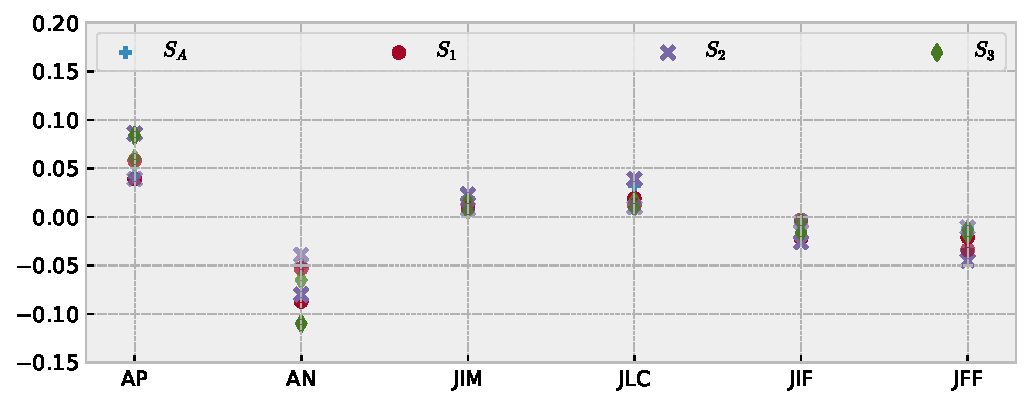
\includegraphics[width=\textwidth]{lc-global-comparison-indicators-means}}\qquad
	\subfloat[Desviaciones típicas]{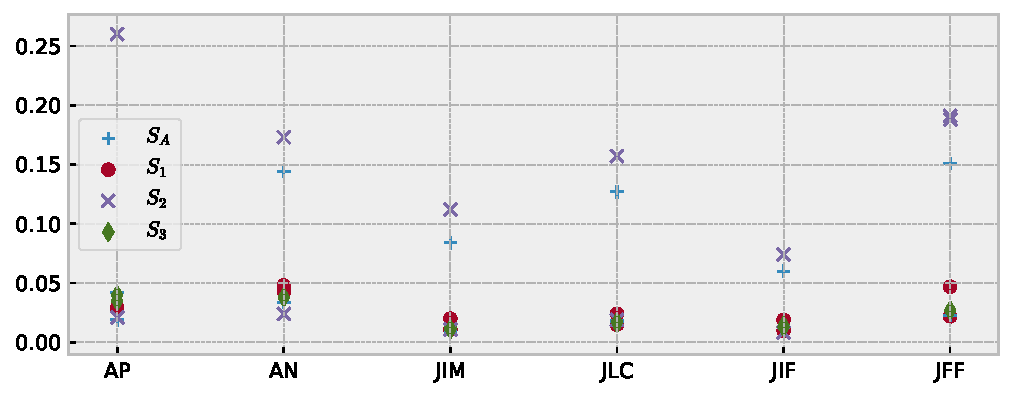
\includegraphics[width=\textwidth]{lc-global-comparison-indicators-stds}}\qquad
	\caption[Medias y desviaciones típicas de los indicadores del modelo longitudinal]{Media y desviación típica de cada uno de los indicadores planteados para el modelo longitudinal.}
	\label{fig:lc-global-comparison-indicators}
\end{figure}

Del resto de sujetos, sin embargo, no se encuentran demasiadas discrepancias, sino que se mantienen en un nivel similar al del resto de variables. Podemos concluir que los valores entre simulación y realidad son muy similares entre sí, y que por tanto que los conductores simulados se pueden considerar similares a los reales en este comportamiento en concreto.



\section{Modelo lateral\index{control lateral}}

Para el comportamiento del modelo de cambio de carril\index{lane-change} se usará el número de cambios que se han producido durante el recorrido, ya que podemos considerar las condiciones similares (i.e. flujo de tráfico moderado en ambas direcciones, misma distancia de recorrido y aproximadamente el mismo número de carriles y semáforos durante el recorrido).

En la Tabla~\ref{tbl:lateral-indicators} se muestra un resumen de los indicadores provenientes de los datos de los conductores en los recorridos frente a los valores. En el caso del conjunto global, se ha elegido la media (redondeada a entero en el caso de cambio de carril) de los tres sujetos como estimador de los valores que correspondan para un supuesto conductor medio en ese recorrido. Los valores de los cambios de carril son el numero exacto y no el número de frames que transcurren durante los mismos. Los valores de cambio de carril correspondientes a las simulaciones son la media y la varianza de tres ejecuciones sobre el mismo escenario.

\begin{table*}
	\centering
	\caption[Indicadores de comportamiento lateral real frente a simulado][2em]{Indicadores de comportamiento lateral real frente a simulado.}
	\label{tbl:lateral-indicators}
	\begin{tabularx}{\linewidth}{cYYYYYYYYYYY}
		\toprule
		& & \multicolumn{2}{c}{$S_A$} & \multicolumn{2}{c}{$S_1$} & \multicolumn{2}{c}{$S_2$} & \multicolumn{2}{c}{\textbf{$S_3$}} & \multicolumn{2}{c}{\textbf{$S_S$}}\\
		\multicolumn{2}{l}{}                  & $\mu$     & $\sigma$ & $\mu$    & $\sigma$ & $\mu$     & $\sigma$  & $\mu$    & $\sigma$   & $\mu$    & $\sigma$ \\
		\midrule
		\rowcolor{black!20} \cellcolor{white} \multirow{2}{*}{\textbf{$LC$}}  & R. & $6$     & $1.414$ & $7$     &  -      & $4$     &    -    & $7$     & -       &  -       &  -       \\
		                                                                      & S. & $2$     & $0$     & $2$     & $0$     & $1$     & $0.471$ & $2$     & $0.816$ &  $11$    &  $0.666$ \\
		\rowcolor{black!20} \cellcolor{white} \multirow{2}{*}{\textbf{$RC$}}  & R. & $3.333$ & $0.942$ & $2$     &  -      & $4$     &    -    & $4$     &    -    &  -       &  -       \\
		                                                                      & S. & $1.667$ & $1.700$ & $0.667$ & $0.471$ & $2.333$ & $1.886$ & $0.667$ & $0.943$ &  $12$    &  $2.666$ \\
		\bottomrule
	\end{tabularx}
\end{table*}

Al igual que ocurría con los indicadores del modelo longitudinal, el número medio de cambios de carril es significativamente más alto en el caso del modelo por defecto de \gls{sumo}\index{SUMO}, por lo que podemos afirmar que éste modelo no se aproxima al comportamiento del resto de conductores.

En el caso de los modelos entrenados se observa el caso contrario, que el número de cambios de carril es menor siempre en el modelo estimado. La razón puede deberse a la baja proporción de cambios de carril respecto a los ejemplos donde éste no existe. Este hecho es muy patente en el caso de los cambios de carril a derecha (fila $RC$ de los indicadores de al tabla~\ref{tbl:lateral-indicators}).

Por tanto, en el caso del cambio de carril, los modelos entrenados se han aproximado más a los valores arrojados en las pruebas reales, aunque es probable que se necesiten más datos de casos de cambio de carril para aproximar mejor sus valores.